\documentclass{utart}

\usepackage{graphicx}
\usepackage{enumitem}
\usepackage{plantuml}

\utUseMinted

\title{uos 系统分区差分升级方案}
\author{jouyouyun}

\begin{document}
\utMakeTitle{}{1.0.0}{2021-11-09}

\utMakeChangeLog{
  1.0.0 & 创建 &  & 2021-11-09 \\
  \hline
}
\utMakeTOC

\section{概述}
\subsection{目的}
本文是对统信 uos 操作系统桌面版如何支持分区差分升级的方案设计,以达到以下目的:
\begin{itemize}[leftmargin=4em]
\item 支持按照目录进行升级
\item 系统与应用安装目录分离
\item 增强系统稳定性
\item 完善系统更新和回滚方案
\end{itemize}

\subsection{背景}
统信 uos 是基于 debian 衍生的商业版本,在系统升级、包管理等方面都延续了 debian 的规则。同样,系统与应用的文件也安装在相同的目录,并且系统与应用之间依赖复杂,不利于系统灵活的更新。

统信 uos 目前采用 A/B 分区的机制实现系统更新和回滚,需要为根分区创建一个相同大小的影子分区,用于系统更新前的系统备份,而备份的系统则用于回滚。此种机制存在以下问题:
\begin{itemize}[leftmargin=4em]
\item 占用硬盘空间,需额外创建一个与根分区等大的分区
\item 分区容量扩充不易,需要同时扩充根分区和影子分区
\item 分区容量耗尽风险,由于根分区安装文件的不确定性,当安装大量软件时会耗尽分区容量
\end{itemize}

因此,我们需要从系统结构、系统分区、系统更新上重新设计一套方案,来增强系统稳定性,满足系统自由升级、易于回滚的要求。

\subsection{术语说明}
\begin{itemize}[leftmargin=4em]
\item hardlink:硬链接,将文件系统中的文件与名称相关联,允许同一文件使用多个硬链接,不支持跨分区或目录的链接。
\item ostree:是一个用于对Linux操作系统进行版本更新的系统,它可以被视为 "面向操作系统二进制文件的git" 。通常用来做操作系统项目的持续交付。
\end{itemize}

\section{方案设计}
\subsection{结构设计}
\begin{center}
  \begin{adjustbox}{scale=0.55}
    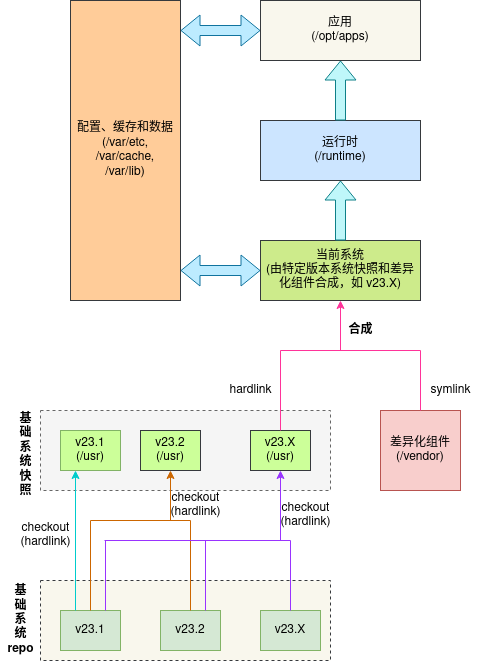
\includegraphics{./uos_structure_design.png}
  \end{adjustbox}

  图 2-1 系统结构
\end{center}

统信 uos 操作系统将由以下部份组成:
\begin{itemize}[leftmargin=4em]
\item 基础系统 repo

  基于 ostree 构建的 repo,内容包含内核、通用驱动、通用服务、DDE 等,是一个能正常运行 DDE 的最小集合,安装到 \texttt{/uos/repo/} 目录。
\item 基础系统快照

  由 repo checkout 生成,利用 hardlink 特性减少磁盘占用,快照文件存储在 \texttt{/uos/snapshot/<version>} , \textbf{必需与 repo 在同一分区} 。
\item 差异化组件

  由差异化的设备驱动、定制的服务、厂商服务组成,如 Nvidia 驱动、杀毒软件等,通过设置 \texttt{PREFIX=/vendor} 将文件安装到 \texttt{/vendor} ,挂载到数据分区,补充基础系统缺失的功能。
\item 当前系统

  由特定版本的基础系统快照和差异化组件合并生成,合并的文件安装在 \texttt{/usr} 目录。合并时系统快照内的文件使用 hardlink 关联,差异化组件通过 symlink 关联。

  当系统快照版本指向发生改变或差异性组件变更时,需要执行合并操作,生成当前系统。合并操作在关机或开机流程中执行。
\item 配置、缓存和数据

  为了保证系统的稳定,\texttt{/etc, /usr} 被设计为静态文件目录,即只能够在 OEM、安装和管理员手动操作时被修改,不允许在运行时被系统或应用修改。

  需要在运行时被修改的文件迁移至数据分区。
\item 运行时环境

  安装到 \texttt{/runtime} ,挂载到数据分区。
\item 应用

  商店及三方厂商的应用,文件安装到 \texttt{/opt/apps} ,挂载到数据分区。
\end{itemize}

基础系统更新时需要兼容已发布的差异化组件,由 uos 确保兼容性。同样,差异化组件升级时应兼容已发布的基础系统,由差异化组件的供应商保证兼容性。

差异化组件内的软件可以发起合入基础系统的申请,由其供应商发起,经过 uos 评审同意后,合入基础系统,并从差异化组件列表里移出。

\subsection{关键技术}
\subsubsection{分区方案}
uos 将分为三个分区:根分区、数据分区、ESP,各分区功能如下:
\begin{itemize}[leftmargin=4em]
\item 根分区:存储基础系统 repo、基础系统快照和当前系统的文件,只读挂载,使用 ext4 文件系统。
\item 数据分区:存储差异化组件、运行时、应用和数据,读写挂载,使用 btrfs 文件系统。
\item ESP:EFI 分区,仅存储 EFI 文件,只读挂载,使用 fat32 文件系统。
\end{itemize}

交换分区使用交换文件取代,便于容量变更和 hibernate 时加密,增强灵活性。

基础系统 repo 和快照存储于根分区中,而差异化组件目录、运行时环境目录、应用目录通过 \texttt{mount bind} 到数据分区。

通过上述分区和挂载方式,将基础系统与其它软件的文件分离,保证了基础系统内的文件不受其它软件的影响。

\subsubsection{基础系统管理方案}
为了便于对基础系统的管理、更新,基础系统基于 ostree 构建为一个 repo,发布时导出为压缩文件(tar.gz),可直接释放为基础系统。

基础系统每一次的更新都创建相关的 branch,通过对 branch 的操作来实现对基础系统的管理。

在完成新 branch 创建后,通过 checkout 操作将 branch 中的内容检出到指定的目录,即可生成对应的基础系统快照。

\subsubsection{当前系统合并生成方案}
由于存在部份第三方软件在代码中写死了配置文件或数据文件的路径,所以设计了这个合并功能,以增强对第三方软件的兼容。

当前系统的生成需要指定系统快照的版本,确定版本后,将对应版本的系统快照文件 hardlink 到 /usr.new 目录。
然后在此基础上将差异化组件内的文件以 symlink 的方式合并到 /usr.new 中,最后将 /usr.new 重命名为 /usr 。

如快照和差异化组件中分别存在以下文件:
\begin{minted}{shell}
# tree v23.1
v23.1
└── usr
    ├── bin
    │   └── htop
    ├── etc
    │   └── fstab.conf
    └── share
        └── htop

# tree vendor
vendor
├── bin
│   └── pkg1
├── etc
│   └── pkg1
│       └── default.conf
└── usr
    └── share
        └── pkg1
            └── pkg1.md
\end{minted}

合并后的目录则如下(不包含快照和差异化组件):
\begin{minted}{shell}
# tree .
.
├── bin -> usr/bin
├── etc -> usr/etc
├── usr
│   ├── bin
│   │   ├── htop
│   │   └── pkg1 -> ../../vendor/bin/pkg1
│   ├── etc
│   │   ├── fstab.conf
│   │   └── pkg1 -> ../../vendor/etc/pkg1
│   └── share
│       ├── htop
│       │   └── README.md
│       └── pkg1 -> ../../vendor/usr/share/pkg1
\end{minted}

\subsubsection{更新和回滚方案}
本方案会为每一次的系统更新生成对应的版本快照,通过对快照的切换实现系统的更新和回滚。

\begin{center}
  \begin{adjustbox}{scale=0.55}
    \begin{plantuml}
      @startuml
      start
      :用户手动或系统自动更新;
      :下载更新文件;
      :标记状态为更新下载完成;
      if (询问是否更新系统) then (NO)
      stop
      else (YES)
      :启动更新模式;
      note right
      退出当前会话,进入更新模式,
      终止非更新模式白名单程序。
      end note
      :解压更新文件;
      :为更新文件创建branch;
      note right
      将更新文件解压到 cache 目录,
      重新挂载根分区为读写,
      使用 ostree commit 添加更新文件,
      并创建新 branch。
      end note
      :标记状态为基础系统更新完成;
      :创建版本快照;
      :标记状态为快照创建完成;
      :切换当前系统到新版本;
      :合并生成新系统;
      :标记状态为系统合并完成;
      :重启;
      endif
      stop
      @enduml
    \end{plantuml}
  \end{adjustbox}

  图 2-2 更新流程
\end{center}

重启之后进入新系统,根据用户反馈或自检确定新系统是否功能正常,若正常则标记状态为更新完成;若不正常,则标记状态为准备回滚,并传入上一个快照版本。
然后进入更新模式,重新生成系统,生成后,则标记状态为更新完成,并重启。

系统启动时,initramfs 检查更新状态,当状态不为更新完成时,根据系统配置决策是否继续剩余流程。

\subsubsection{数据分区备份方案}
数据分区采用 btrfs 文件系统,目的是使用其快照特性。差异化组件和应用都安装在此分区,当检测到差异化组件或重要应用进行更新时,会主动提醒用户创建快照,便于在新版本出现异常时进行数据回滚。

系统会内置一份重要应用列表,以此判断更新中是否包含重要应用。

\subsubsection{配置、缓存、数据存储规范}
uos 将文件分为静态文件和可变文件,静态文件是指只能在 OEM、更新和管理员手动操作时才能更改的文件,这些文件默认只读。除此之外的文件则为可变文件。

/etc 目录因包含了系统启动相关的重要配置,错误更改后会导致系统启动失败,影响系统稳定性。因此将其设计为静态文件目录,但一些服务和应用也会使用 /etc 目录作为默认配置目录,并可能会在运行时修改。

这与 uos 的设计违背,因此需要对配置、缓存和数据存储目录做要求:
\begin{itemize}
\item 配置:/var/etc 存储系统级配置,\$HOME/.config 存储用户级配置;
\item 缓存:/var/cache 存储系统级缓存, \$HOME/.cache 存储用户级缓存;
\item 数据:/var/lib 存储系统级数据, \$HOME/.local 存储用户级数据;
\end{itemize}

\end{document}
